Seja $G = (V,E)$ o grafo da instância do problema e $c_e$ o custo de uma aresta $e \in E$.
    Definimos a função $c(u,S)$ que é definida para um vértice $u$ e um conjunto $S$ de vértices  por,
    \[ c(u,S) = \min_{v\in S} c_{uv}
        \]
    A ideia desse algoritmo guloso se concentrará em, a cada iteração, escolher o vértice $u$ tal que $c(u,C)$ seja o maior possível, sendo $C$ o conjunto dos centros de cluster escolhidos até aquele momento.

    \begin{algorithm}
		\caption{G$(G,c,k)$}
        \label{k-center:guloso}
        \begin{algorithmic}[1]
			\State Escolha arbitrariamente $u \in V$.
            \State $C \gets \{u\}$.
            \While{$|C| \leq k$}
            \State $v \gets \arg\max_{j \in V} c(j,C)$
            \State $C \gets C \cup \{v\}$
            \EndWhile 
			\State Devolva $C$.
		\end{algorithmic}
	\end{algorithm}
    
    \begin{theorem}
        O algoritmo {\sc G}$(G,c,k)$ é uma $2$-aproximação do problema dos $k$-centros.
    \end{theorem}
    \begin{proof}
        Primeiramente, vamos mostrar que o algoritmo é polinomial. A única linha que não é claramente polinomial é a linha $5$. Para cada vértice $v \in V$, vamos olhar o custo de $|C|$ arestas. Como $|C| \leq |V|$, então iremos olhar o custo de no máximo $|V|^2$ arestas a cada iteração. Assim, nosso algoritmo roda em tempo $O(k|V|^2)$. \\
        Seja $C^*$ um conjunto ótimo de centros de cluster para $I(G,c,k)$. Vamos mostrar que raio$(C) \leq 2\opt(I) $. Perceba que o custo entre dois vértices quaisquer de um mesmo cluster de $C^*$ é no máximo $2\opt(I)$, uma vez que vale a desigualdade triangular.\\ 
        Se há um vértice de $C$ em cada cluster de $C^*$, todos os vértices estão ligados com uma aresta de custo no máximo $2\opt(I)$ a um centro de cluster de $C$. Então raio$(C) \leq 2\opt(I)$. \\
        Senão, suponha sem perda de generalidade que $C_{i-1} = \{ u_1,u_2,\ldots,u_{i-1}\}$ é o $C$ ao final da iteração $i-1$ e cada $u_j$ está em um cluster diferente de $C^*$. Seja $u_i$ o vértice escolhido na iteração $i$ e suponha que ele está no mesmo cluster que um vértice $u_j$ para algum $j=1,\ldots,i-1$. Então, $c(u_i,C_{i-1}) \leq c(u_iu_j) \leq 2\opt(I)$. Como $u_i$ maximiza $c(v,C_{i-1})$, então raio$(C) \leq 2\opt(I)$.
    \end{proof}
    Esse algoritmo é de autoria de Gonzalez~\cite{GONZALEZ1985293}.
    Vamos mostrar que essa análise é justa, ou seja, existe uma instância $I(G,c,k)$ em que o algoritmo devolve uma solução $C$ tal que raio$(C) = 2 \opt(I)$. \\
    O grafo $G$ contém pelo menos $k+2$ vértices e as arestas têm custo 1 ou 2. O grafo induzido pelas arestas de custo 1 é uma estrela, como mostrado na figura abaixo.
    \[
    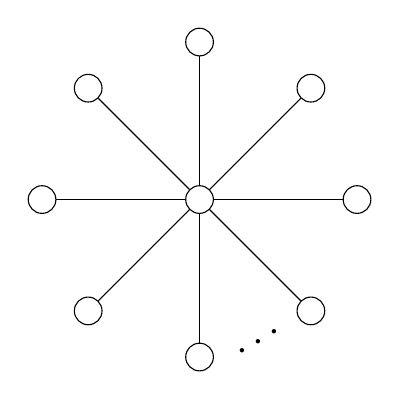
\begin{tikzpicture}
        % Number of outer vertices in the star
        \def\n{8}
        
        % Radius of the star
        \def\r{2cm}
        
        % Rotation angle
        \def\rotationangle{90}
        
        % Draw the central vertex
        \draw (0,0) node[circle, draw, minimum size=10pt, inner sep=1.5pt] (center) {};
        
        % Draw the outer vertices, rotated
        \begin{scope}[rotate=\rotationangle]
          \foreach \i in {1,...,\n} {
            \draw (\i*360/\n:\r) node[circle, draw, minimum size=10pt, inner sep=1.5pt] (\i) {};
          }
        \end{scope}
        
        % Connect the central vertex to every outer vertex
        \foreach \i in {1,...,\n} {
          \draw (center) -- (\i);
        }
        \draw (4) node[shift={(0.75,0.2)}] {\rotatebox{30}{\scalebox{1.5}{$\ldots$}}} (4);
      \end{tikzpicture}
      \] \\
      Claramente, o raio de uma resposta ótima dessa instância é 1 e inclui o vértice do centro da estrela como um dos centros de cluster. \\
      Note que se, no algoritmo guloso, o vértice escolhido arbitrariamente for algum dos vértices da ponta dessa estrela o vértice do centro nunca será escolhido, uma vez que ele nunca maximizará a função $c(j,C)$. Assim, serão escolhidos apenas vértices da ponta da estrela e como temos pelo menos $k+1$ delas, sempre existirá um vértice ligado ao centro do seu cluster com uma aresta de custo 2.